\documentclass{beamer}
\usetheme{default}
\usepackage{graphicx}

\begin{document}
\begin{frame}{Angular correlation Function}
	$$F = 1 + a \frac{\boldsymbol{p_e}\cdot\boldsymbol{p_\nu}}{E_eE_\nu} + \frac{\boldsymbol{J}}J\cdot\left(A \frac{\boldsymbol{p_e}}{E_e} + B \frac{\boldsymbol{p_\nu}}{E_\nu} + D \frac{\boldsymbol{p_e}\times\boldsymbol{p_\nu}}{E_eE_\nu}\right)$$
	
	
	Spherical Coordinates ($\boldsymbol{J}$ zAxis)
	
	$\boldsymbol{\beta_e} = (r=\beta_e;\theta=\theta_e;\phi=0),\quad\cos(\theta_e) \equiv z_e$
	
	$\boldsymbol{\beta_\nu} = (r=1;\theta=\theta_\nu;\phi=\phi),\quad\cos(\theta_\nu) \equiv z_\nu$
	
	
	$$\boldsymbol{\beta_e}\cdot\boldsymbol{\beta_\nu} = \beta_e(\cos\theta_e\cos\theta_\nu + \sin\theta_e\sin\theta_\nu\cos\phi) =$$
	$$ \beta_e(z_ez_\nu + \sqrt{1-z^2_e}\sqrt{1-z^2_\nu}\cos\phi)$$
	$$\boldsymbol{\beta_e}\cdot\boldsymbol{j} = \beta_e\cos\theta_e=\beta_ez_e$$
	$$\boldsymbol{\beta_\nu}\cdot\boldsymbol{j} = \cos\theta_\nu=z_\nu$$
	$$\boldsymbol{j}\cdot(\boldsymbol{\beta_e}\times\boldsymbol{\beta_\nu})=\beta_e\sin\theta_e\sin\theta_\nu\sin\phi=\beta_e\sqrt{1-z^2_e}\sqrt{1-z^2_\nu}\sin\phi$$
\end{frame}	
	
\begin{frame}{Single Variable: A}
\begin{figure}
	\centering
	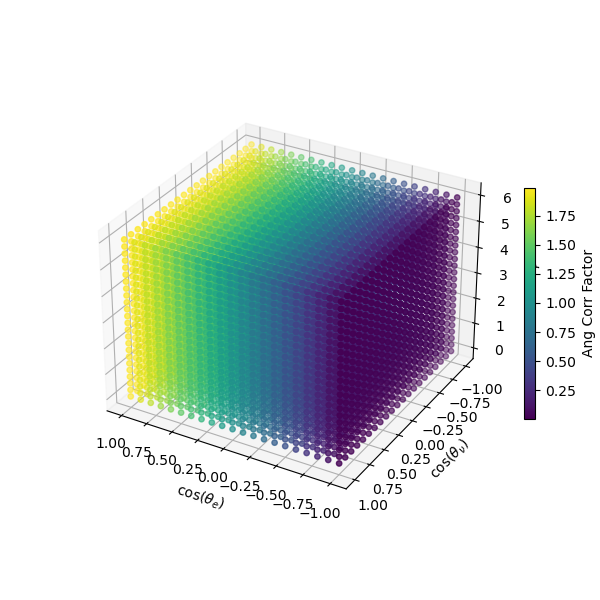
\includegraphics[width=0.4\paperwidth]{plots/A_3D_image.png}
	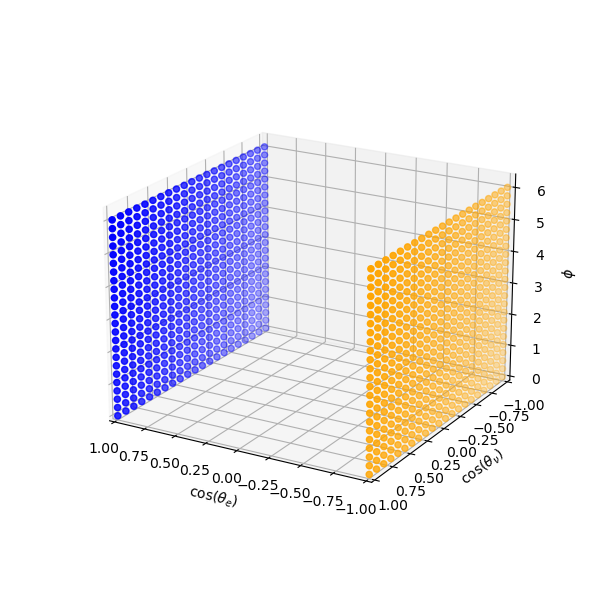
\includegraphics[width=0.4\paperwidth]{plots/A_max_min.png}
	\caption{(Right) Values of the angular correlation Factor with A = 1, E = 5000 keV and rest of variables 0. (Left) Location of maximum (blue, value = 1.995) and minimum (orange, value = 0.005)}
\end{figure}
\end{frame}
\begin{frame}{Single Variable: A}
	\begin{figure}
		\centering
		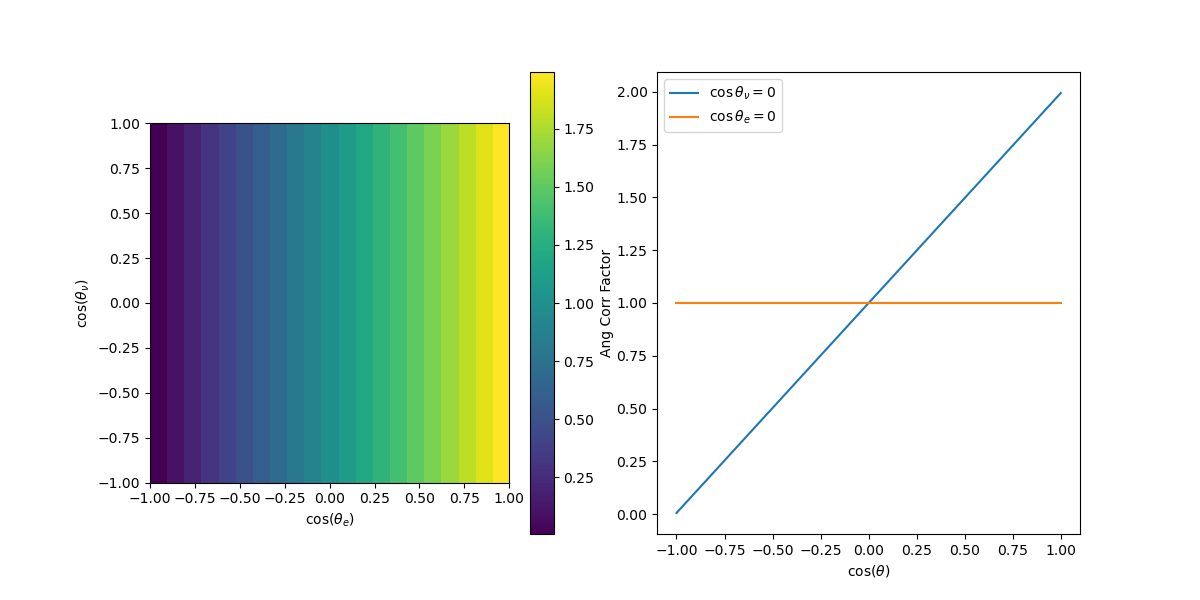
\includegraphics[width=0.8\paperwidth]{plots/crosssections_A.png}
		\caption{(Right) 2D projection of previous 3D image at any $\phi$ (Left) 1D projections at any $\phi$, and either $z_e = 0$ or $z_\nu = 0$ }
	\end{figure}
\end{frame}

\begin{frame}{Single Variable: B}
\begin{figure}
	\centering
	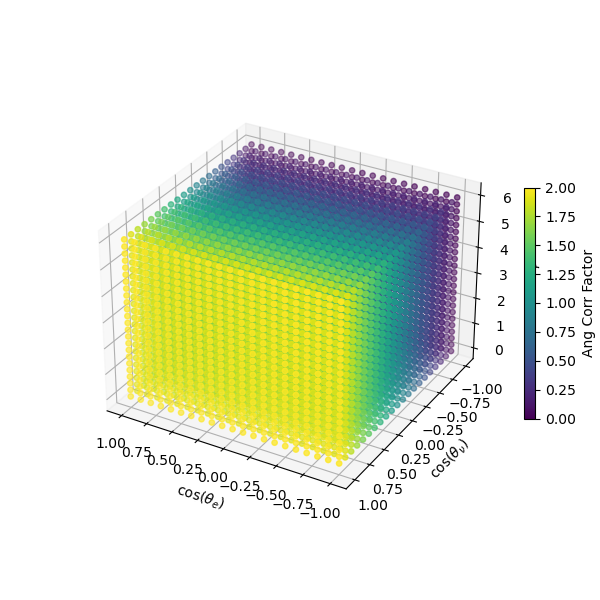
\includegraphics[width=0.4\paperwidth]{plots/B_3D_image.png}
	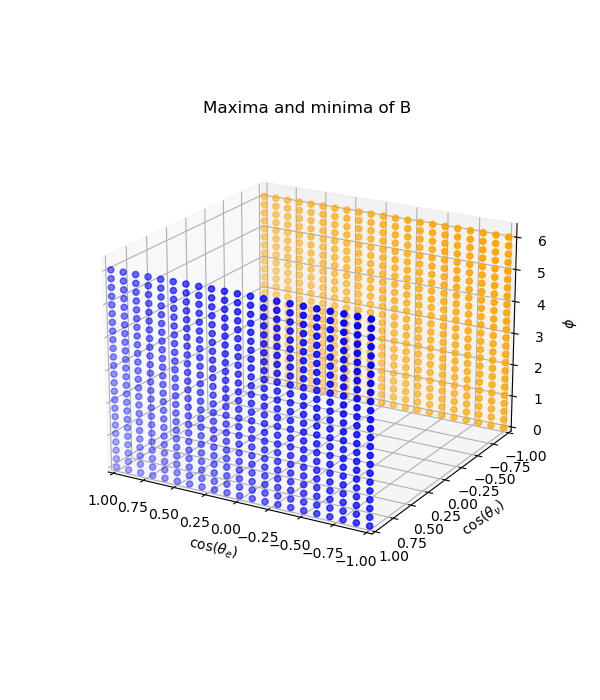
\includegraphics[width=0.4\paperwidth]{plots/B_max_min.png}
	\caption{(Right) Values of the angular correlation Factor with B = 1, E = 5000 keV and rest of variables 0. (Left) Location of maximum (blue, value = 2) and minimum (orange, value = 0)}
\end{figure}
\end{frame}
\begin{frame}{Single Variable: B}
	\begin{figure}
		\centering
		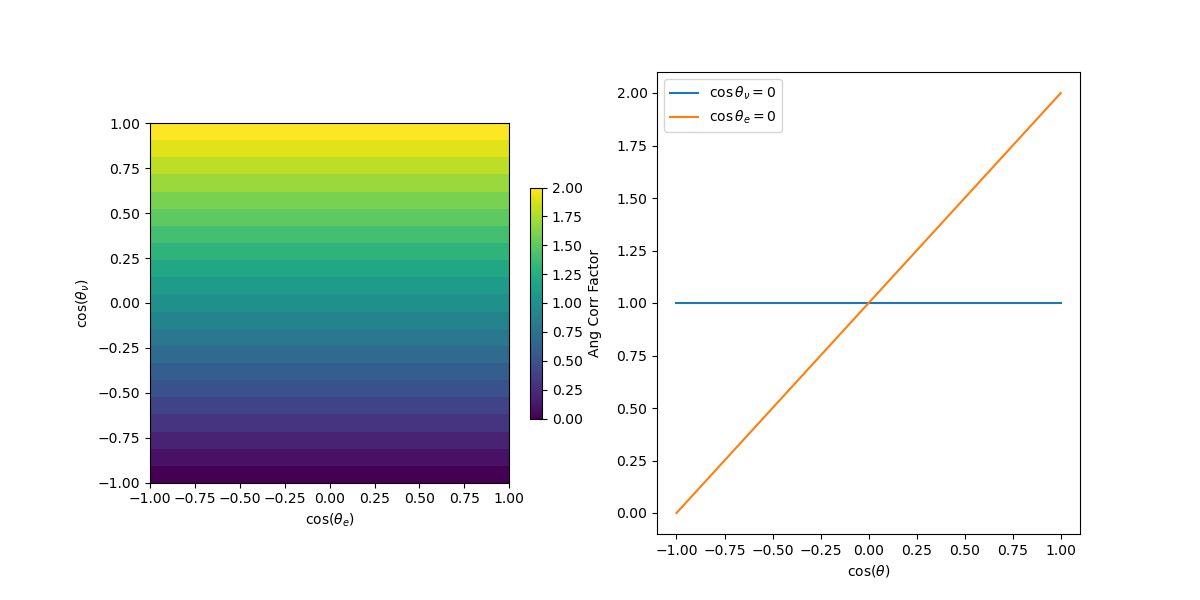
\includegraphics[width=0.8\paperwidth]{plots/crosssections_B.png}
		\caption{(Right) 2D projection of previous 3D image at any $\phi$ (Left) 1D projections at any $\phi$, and either $z_e = 0$ or $z_\nu = 0$ }
	\end{figure}
\end{frame}

\begin{frame}{Single Variable: a}
\begin{figure}
	\centering
	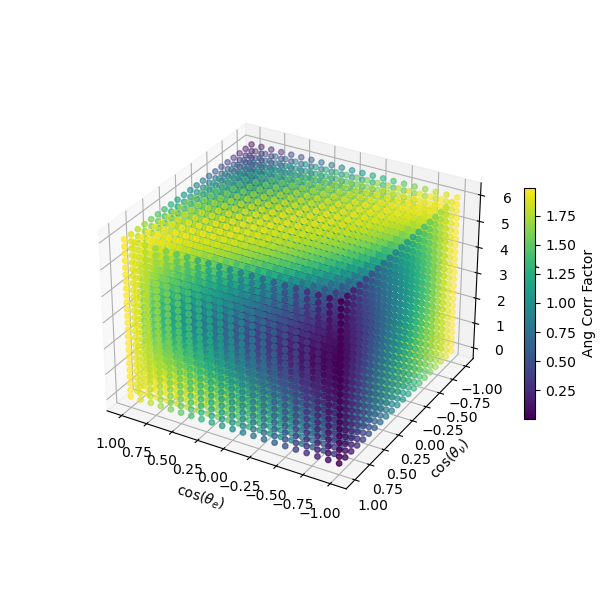
\includegraphics[width=0.4\paperwidth]{plots/a_3D_image.png}
	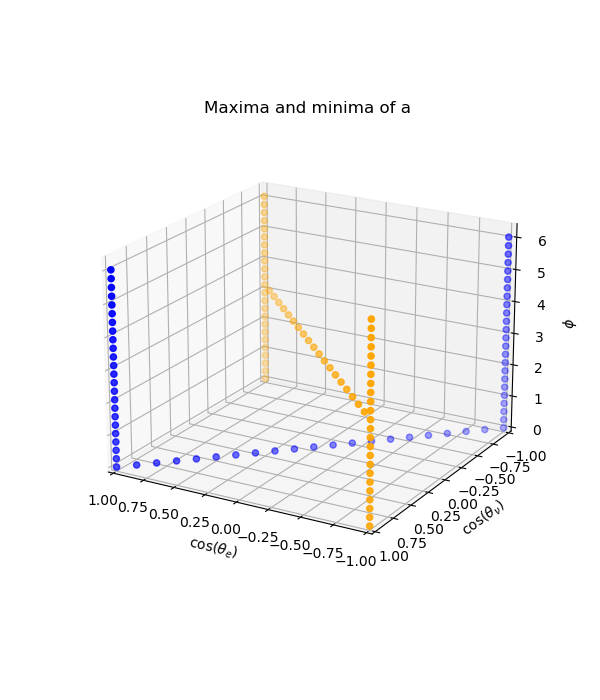
\includegraphics[width=0.4\paperwidth]{plots/a_max_min.png}
	\caption{(Right) Values of the angular correlation Factor with a = 1, E = 5000 keV and rest of variables 0. (Left) Location of maximum (blue, value = 1.995) and minimum (orange, value = 0.005)}	
\end{figure}
\end{frame}
\begin{frame}{Single Variable: a}
	\begin{figure}
		\centering
		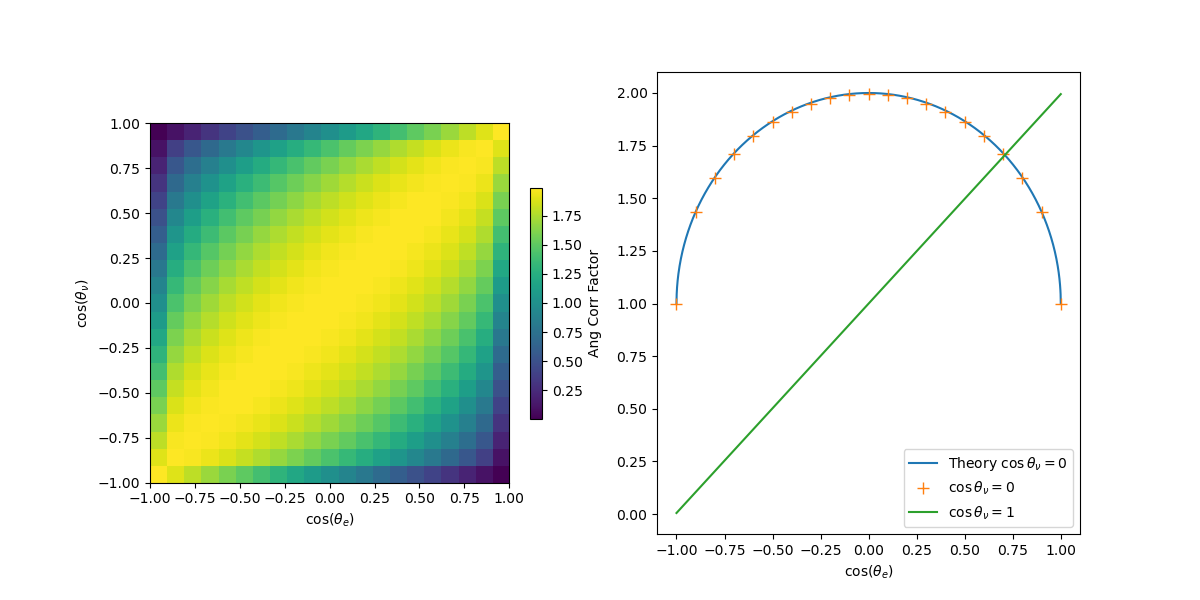
\includegraphics[width=0.8\paperwidth]{plots/crosssections_a.png}
		\caption{(Right) 2D projection of previous 3D image at $\phi = 0$ (Left) 1D projections at $\phi=0$, and either $z_\nu = 0$ or $z_\nu = 1$ }
	\end{figure}
\end{frame}

\begin{frame}{Single Variable: D}
\begin{figure}
	\centering
	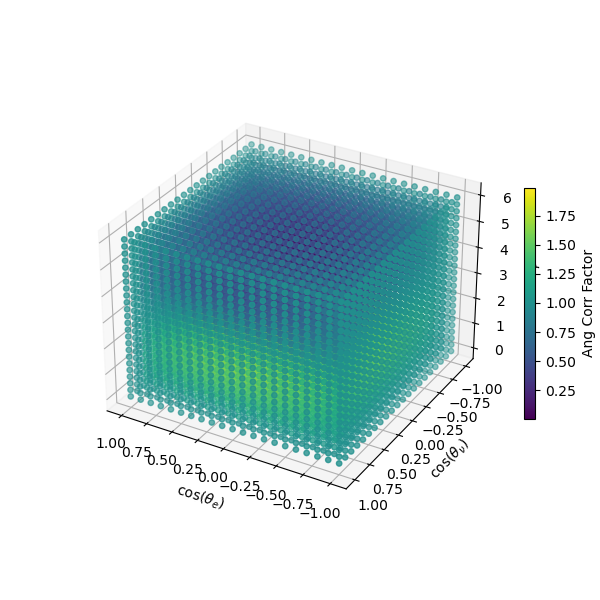
\includegraphics[width=0.4\paperwidth]{plots/D_3D_image.png}
	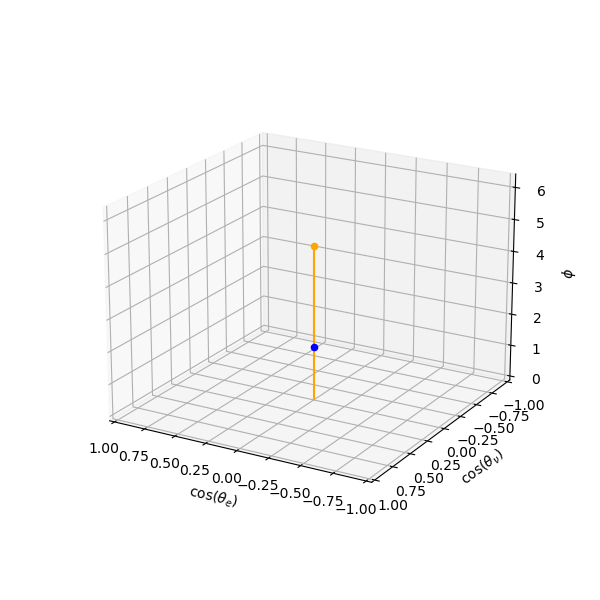
\includegraphics[width=0.4\paperwidth]{plots/D_max_min.png}
	\caption{(Right) Values of the angular correlation Factor with D = 1, E = 5000 keV and rest of variables 0. (Left) Location of maximum (blue, value = 1.995) and minimum (orange, value = 0.005)}	
\end{figure}
\end{frame}
\begin{frame}{Single Variable: D}
	\begin{figure}
		\centering
		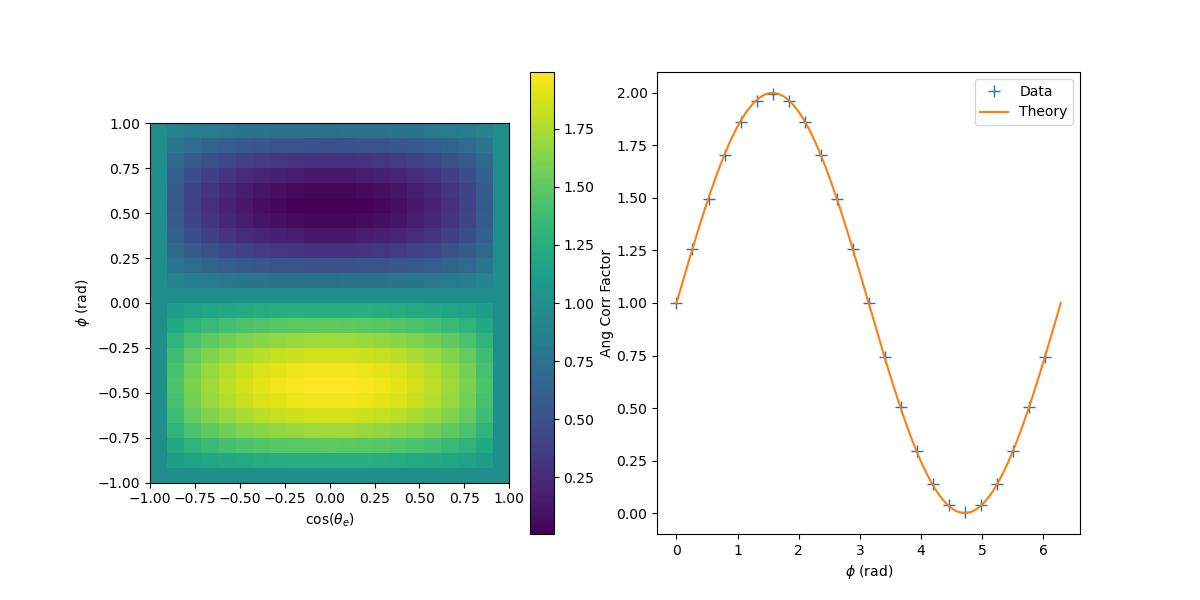
\includegraphics[width=0.8\paperwidth]{plots/crosssections_D.png}
		\caption{(Right) 2D projection of previous 3D image at $z_\nu = 0$ (Left) 1D projection at $z_\nu = 0$ and $z_\nu = 0$ }
	\end{figure}
\end{frame}

\end{document}
